%scrrprt ist eine Klasse für Berichte und längere Arbeiten
\documentclass[11pt,a4paper]{scrreprt}
%ermöglicht die Eingabe von Umlauten usw. ohne Codierung
\usepackage[utf8]{inputenc}
%Schriften werden mit einer passenden Kodierung für europäische Zeichen ausgegeben
\usepackage[T1]{fontenc}
%Passt Dokumentelemente an die Konventionen der deutschen Sprache (neue Rechtschreibung) an, z.b. Datumsangaben, Silbentrennung
\usepackage[ngerman]{babel}
%Grafikpaket
\usepackage{graphicx}
\usepackage{scrpage2}
\usepackage{color}
\usepackage{array}
\usepackage{booktabs}
\usepackage{hyperref}
\definecolor{light-gray}{gray}{0.85}
\renewcommand\emph[1]{\colorbox{light-gray}{\texttt{#1}}}
\pagestyle{scrheadings}
\clearscrheadfoot
%\Chapter sorgt dafür, dass kein Seitenvorschub auftritt.
\makeatletter
\newcommand\Chapter{%
                    \par\vspace{0.01cm}% anpassen
                    \global\@topnum\z@
                    \@afterindentfalse
                    \secdef\@chapter\@schapter}
\makeatother


\begin{document}
\begin{titlepage}
	\centering
	{\scshape\LARGE Universität Leipzig \par}
	\vspace{1cm}
	{\scshape\Large Information Retrieval Laborprojekt \par}
	\vspace{2cm}
	{\huge\bfseries Evaluation der Geocache-Suchmaschine \par}
	\vspace{2cm}
	{\Large\itshape Steven Lehmann, Fabian Ziegner, Christian Schlecht \par}
	\vfill
	supervised by \par
	Jun.-Prof. Dr.~Martin \textsc{Potthast}
	\vfill
	{\large \today \par}
\end{titlepage}
\tableofcontents

\ihead{11.12.2017}
\ohead{Gruppe Geocache-Search}
\cfoot{\pagemark}

\Chapter{Begriffserklärungen}
\section{Geocaching}
Unter Geocaching wird eine Art Schnitzeljagd verstanden. Das Wort leitet sich vom lateinischen $\gamma$$\widetilde{\eta}$, gē, stehend für ``Erde`` und dem englischen ``cache`` für ``geheimes Lager`` ab. Ziel ist es, mit Hilfe von GPS-Koordinaten und/oder veröffentlichen Tipps einen versteckten Behälter - den sogenannten ``Geocache`` (auch kurz ``Cache``)  - zu finden. In der Regel beinhaltet dieser Behälter ein Logbuch, in welches sich die Geocacher bei erfolgreicher Suche eintragen können. Zusätzlich, sofern es die Größe des Behälters hergibt, sind oftmals kleine Gegenständen zum Tausch vorhanden. Wichtig ist es, während der gesamten Zeit möglichst unentdeckt zu bleiben, sodass der Cache stets verborgen bleibt. Nach Beendigung der Suche wird der Cache wieder an seine ursprüngliche Position gebracht.

Es gibt eine ganze Reihe Arten von Geocaches. Vom einfachen traditionelle Caches, über Multi-Caches und Rätsel-Caches bis hin zu virtuellen Caches können Suchen veranstaltet werden.

Fairness wird beim Geocaching groß geschrieben. Personen, die den Cache veröndern, mutmaßlich zerstören, entfernen oder Dinge daraus stehlen wird größter Missmut entgegengestellt.

\Chapter{Motivation}
\section{Domäne}
\subsection{Geocaching als Sport}
Geocaching erfreut sich zunehmender Beliebtheit unter der Bevölkerung, obwohl es in gewissem Sinne das Ziel ist, geheim zu agieren. Dieser Sport kann von Menschen aller Altersgruppen und körperlicher Verfassung betrieben werden, da in praktisch jeder Region (Wald, Stadt, Parkanlagen, Gebirge, \dots) Caches versteckt und gefunden werden können. Unterbewusst wird dadurch die Gesundheit gefördert. Aus dieser Hinsicht ist der Sport in jedem Fall zu unterstützen. 

\subsection{technischer Stand}
Mittlerweile wird Geocaching durch das Internet stark unterstützt und vereinfacht. Während in den Anfängen (1980er Jahre) die Hinweise und Koordinaten meist verbal oder handschriftlich verbreitet wurden, gibt es heutzutage diverse Plattformen und Foren, um sich auszutauschen. Zu den bekanntesten gehören hier \href{geocaching.com}{geocaching.com} und \href{opencaching.de}{opencaching.de} im deutschsprachigen Raum. Diese Seiten agieren im Wesentlichen als Foren zum Austausch mit anderen Cachern. Sie bieten zwar die Möglichkeit der Suche, jedoch wird hierbei auf eine Datenbank zurückgegriffen, aus welcher mittels SQL-Anweisungen Suchanfragen bearbeitet werden. Wir haben keinen Anbieter feststellen können, der bei der Suche Methoden des Information Retrieval, d.h. Verwendung eines Index und Retrieval-Modells, anwendet. An dieser Stelle wird im Rahmen dieses Projekts prototypisch gearbeitet. 

\section{Dokumentkorpus}
Die Geocaching Suchmaschine soll für Geocaches in Deutschland angewendet werden. Aus diesem Grund wurde als Dokumentkorpus eine Sammlung von allen \footnote{Stand 24.04.18} Geocaches in Deutschland, welche auf \href{opencaching.de}{opencaching.de} veröffentlicht sind, gewählt. Der Korpus beläuft sich damit auf eine Größe von ca. 20.000 Caches. Aufgrund des Mehraufwandes eines Web-Crawls wurden diese manuell heruntergeladen. Die Dokumentsammlung kann also als statisch betrachtet werden. 

\subsection{Dokumentstruktur}
Jedes Dokument kann von opencaching.de in diversen verschiedenen Formaten heruntergeladen werden, darunter auch direkt von GPS-System verwertbare Formate. Aufgrund der Vollständigkeit der Information wurden in diesem Rahmen Caches im .txt-Format verwendet. 

Das Dokument wird bereits beim Herunterladen in eine wohlgeformte Struktur gebracht. Die Abbildung \ref{img:struktur} zeigt einen Ausschnitt. Es lässt sich eine Art Key-Value-Struktur erkennen, welche das spätere Parsing der Dokumente vereinfacht, sodass eine maximale Korrektheit gewährleistet werden kann.
Interessant ist hierbei, dass durch dieses Dokument sämtliche Informationen aus der Web-Darstellung übernommen werden, die Informationen sind also a prior vollständig.

\begin{figure}
	\centering
	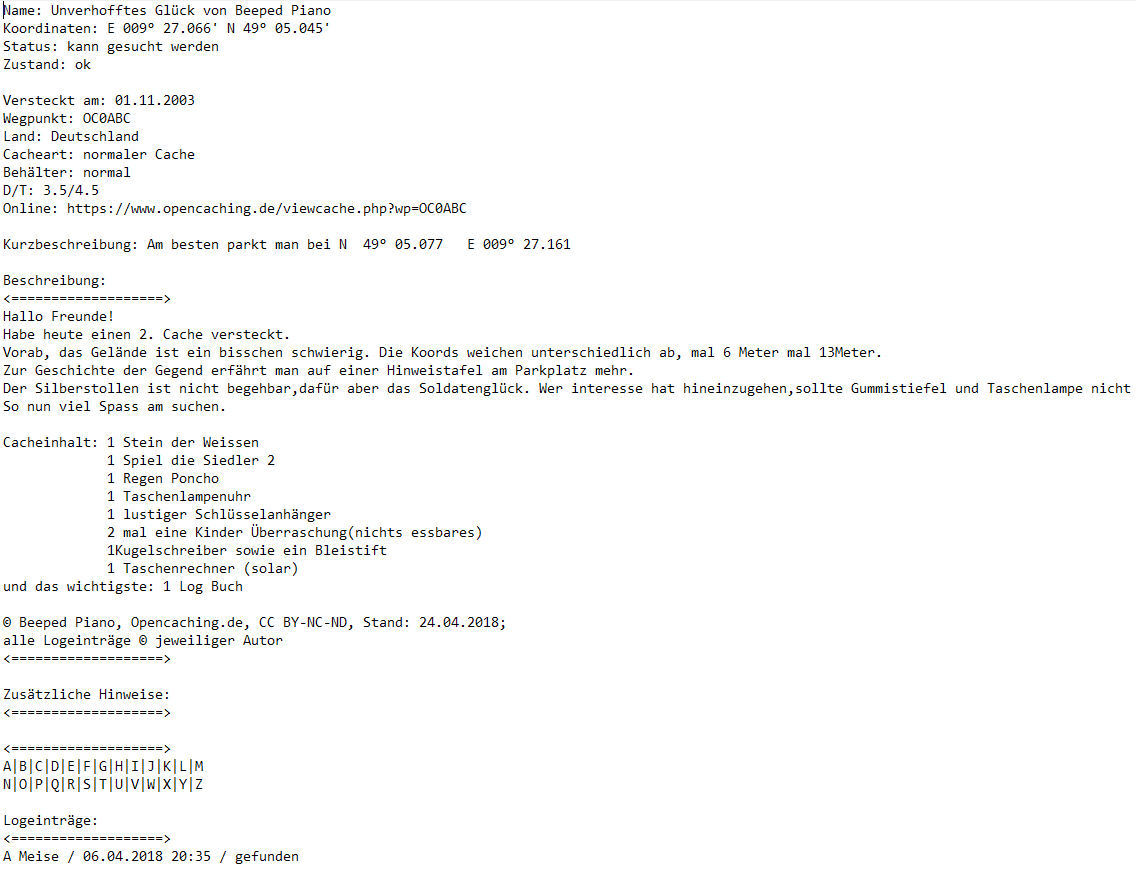
\includegraphics[height=0.6\textheight]{cache_struktur.png}
	\caption{Dokumenstruktur eines Geocaches}
	\label{img:struktur}
\end{figure}


\Chapter{Architektur}
\section{Grobstruktur}
Die Geocache Suchmaschine funktioniert nach dem Client-Server Prinzip. Als Programmiersprachen wurde für das Backend Java und für den Client natives HTML/CSS und JavaScript verwendet. Das Frontend empfängt angeforderte Daten vom Server (im Wesentlichen Beantwortung der Suchanfragen) über eine REST-Schnittstelle, welche mit Hilfe des Jersey - Frameworks \footnote{https://jersey.github.io/} erstellt wurde.

\section{Backend}
Der Server wird als Webapplikation mit Hilfe einer Tomcat-Instanz als Container betrieben. Die Suchmaschine wurde mittels Apache Lucene \footnote{http://lucene.apache.org/} implementiert. Daneben existiert eine REST-Schnittstelle zur Kommunikation mit dem Frontend. Im Folgenden werden die einzelnen Bestandteile genauer erläutert.

\section{Kommunikation}
Über das Resource-Package des Servers werden Daten zum und vom Frontend gesendet. Es existieren GET-Requests zum Suchen (sowohl einfache als auch erweiterte Suche) und für das Empfangen von Suggestions. Ein weiterer POST-Request ermöglicht das Übertragen des Loggings an den Server. Die strikte Trennung zwischen Backend und Frontend ermöglicht beispielsweise das einfache Austauschen des Frontends oder die Anbindung an bereits bestehende Services.

\section{Parsing der Dokumente}
Bevor der Index für die Suchmaschine erstellt werden kann, müssen die vorhandenen .txt-Dateien in ein verarbeitbares Format gebracht werden. Aufgrund der Leichtgewichtigkeit und intuitiver Lesbarkeit wird das JSON-Format verwendet.
Jedes Dokument wird zeilenweise in den Parser eingelesen. Anhand der bereits vorhandenen Key-Value-artigen Strukturen (siehe Abbildung \ref{img:struktur}) wird nach den Keys gesucht, diese entfernt, und die übrigen Values, d.h. die eigentlichen Daten, zu einem Java-Objekt zusammengefasst. Die Abbildung \ref{img:objekt} zeigt dieses. 

\begin{figure}
	\centering
	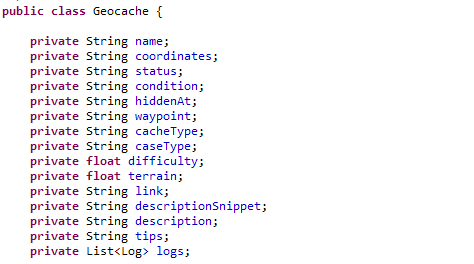
\includegraphics[height=0.3\textheight]{cache_objekt.png}
	\caption{Java Objekt zur Repräsentation eines Caches}
	\label{img:objekt}
\end{figure}

Zuletzt wird dieses Objekt mit Hilfe der org.json Library \footnote{https://github.com/stleary/JSON-java} in ein JSON Objekt überführt und schließlich in eine .json-Datei geschrieben. Der Name der Datei setzt sich aus dem Waypoint-Attribut des Geocaches zusammen, welches eine eindeutige Zuordnung ermöglicht. Dieses Attribut wird bereits durch die Rohdaten von opencaching.de geliefert. \emph{TODO BILD VOM JSON}
Die .txt - Rohdaten werden ab diesem Zeitpunkt nicht mehr benötigt.

\section{Architektur der Suchmaschine}

\subsection{Index}
Der Index wird anhand der zuvor erstellten json - Dateien konfiguriert. Jeder Geocache stellt hierbei ein eigenes Document im Index dar. Analog erhält jedes Attribut des Geocache-Java-Objekts ein eigenes Field. Lediglich auf die Attribute Tipps und Link wird verzichtet, da diese für den Index irrelevante Information enthalten (Tipps sind in Caesar-Chiffre verschlüsselt, Link ist ein HTML-Link auf opencaching.de). Es ist äußert unwahrscheinlich, dass derartige Suchqueries auftreten. Die übrigen Attribute werden mittels 3-Grammen indexiert. Dies ist besonders effizient für einen ``Search-as-you-type``-Ansatz, da Edge-N-Gramme genau den Fluss der Eingabe widerspiegeln. Aus Zeitgründen wurde diese Methode leider nicht mehr umgesetzt.

\subsection{Suche}
 Die Geocache-Suchmaschine ermöglicht zwei Arten der Suche: Zum einen eine standardmäßige Suche mittels einer Query, und desweiteren eine erweiterte Suchmaske, durch welche zusätzliche Suchparameter einbezogen werden können.

\subsubsection{einfache Suche}
Die einfache Suche ermöglicht die Eingabe eines Query-Strings, nach welchem der Index durchsucht werden soll. Es können sowohl die Lucene-Query-Syntax als auch natürlichsprachige Anfragen beantwortet werden. Als QueryParser wird ein \emph{MultiFieldQueryParser} verwendet. Dieser sucht in allen Fields der Dokumente nach der Query. Zuvor werden durch einen GermanAnalyzer sowohl alle ``normalen`` Stoppworte der deutschen Sprache, als auch domänenspezifische Stoppworte, gefiltert. Diese umfassen die Worte ``Geocache`` und ``Cache``, da diese für die Semantik der Suche nicht von Bedeutung sind (nahezu alle Dokumente enthalten das Wort Geocache oder Cache, da diese das Thema sind). Würde man diese Worte nicht filtern, so würden Ergebnisse stark verfälscht werden (nähere Erläuterungen siehe Kapitel \ref{evaluation}). Nach eingänglicher Betrachtung der Dokumente wurde sichtbar, dass zum einen der Name des Caches und zum anderen die Beschreibung die Felder sind, welche die meisten, d.h. die am such-relevantesten, Informationen enthalten. Aus diesem Grunde erhalten der Name einen Boost von $2.5$ und die Beschreibung einen Boost von $1.5$. Denkbar wäre auch ein Boost für die Logs zu etablieren, jedoch enthalten diese bei genauerer Betrachtung vielmals ``nur`` Vermerke über das Auffinden, sowie persönliche Kommentare zu Schönheit des Caches oder Tauschverhalten. Aus diesem Grunde werden die Logs nicht geboostet.

\subsubsection{erweiterte Suche}
Die erweiterte Suche bietet genau wie die einfache Suche die Möglichkeit zur Eingabe eines Query Strings. Zusätzlich dazu können Parameter, welche die Suche verfeinern, angegeben werden (z.B. nur Suche nach bestimmten Cache-Arten). Jeder Parameter repräsentiert dabei ein Field im Document. Für jeden angegebenen Parameter wird ein separater \emph{SimpleQueryParser} verwendet, der im jeweilig korrespondierenden Field sucht. Die Query wird analog zur einfachen Suche verarbeitet. Im letzten Schritt werden nun die einzelnen Queries für die Parameter mit der Suchquery verschmolzen, um im Endeffekt nur eine einzige Suche durchführen zu müssen. Dies geschieht mit Hilfe eines \emph{BooleanQuery.Builder}'s mit dem Junktor \emph{BooleanOccur.MUST}.

\subsection{Suggestions}
Die Suchmaschine besitzt eine Autocompletion in etwas abgewandelter Form als gebräuchlich. Anstatt die Query beim Tippen Wort für Wort zu vervollständigen, werden stattdessen direkt Namen von Caches vorgeschlagen, welche zur aktuellen Eingabe passen. Da in der deutschen Sprache sowohl Prä -  als auch Suffixe verbreitet sind, müssen diese geeignet erkannt werden, um falsche bzw. nicht ausreichend passende Vorschläge auszuschließen. Hierbei wird ein \emph{AnalyzingInfixSuggester} verwendet, welcher von Lucene bereitgestellt wird. Da dieser Suggester einen eigenen Lookup-Index aufbaut, muss Redundanz in Kauf genommen werden. Dieser Index ist jedoch deutlich kleiner als der eigentliche Suchindex, da er lediglich die Namen der Caches indexiert und alle übrigen Informationen ignoriert. Das Ranking des AnalyzingInfixSuggester's erfordert eine Gewichtung. Diese wird anhand der Anzahl der Logs berechnet. Caches, die mehr Logs enthalten, sind stärker frequentiert und damit tendenziell relevanter als Andere mit weniger Logeinträgen. Somit werden diese als Erstes vorgeschlagen.




\Chapter{Evaluation} \label{evaluation}

Zur Evaluation wurden insgesamt 14 Topics erstellt, die exemplarisch die Mehrheit der möglichen Suchanfragen abdecken sollen. Es handelt sich dabei um Stichwortsuchen und Phrasensuchen sowohl mit als auch ohne erweiterte Suchparameter. Für jedes Topic wurden die besten 10 Suchergebnisse evaluiert. Das Relevanzmaß ist \textit{Precision@k} und daraus resultierende \textit{Average Precision}.  Tabelle \ref{table:eval} zeigt die verwendeten Suchquery mit ihren jeweils errechneten Precisions. Es ergibt sich letztendlich eine \textit{Mean Average Precision} von $0.60$.

\begin{table}
\caption{Topics zur Evaluation}
\label{table:eval}
\renewcommand{\arraystretch}{1.5}
\begin{tabular}{cllc}
\toprule
ID 	&	Suchquery							&	Kategorie 				&	Average Precision\\
\midrule
1	&	\textit{Geocache im Wald}					&	Stichwortsuche			&	$1.00$\\
2	&	\textit{sonniger Geocache}				&	Stichwortsuche			&	$0.58$\\
3	&	\textit{Leipzig Auenwald}					&	Stichwortsuche			&	$0.64$\\
4	&	\textit{Fahrrad erreichbar}				&	Phrasensuche			&	$0.62$\\
5	&	\textit{leicht zu finden}					&	Phrasensuche			&	$0.13$\\
6	&	\textit{Cache mit Aussicht}				&	Stichwortsuche			&	$1.00$\\
7	&	\textit{See in Leipzig + cacheType=Multicache}	&	Stichwortsuche mit Parameter	& 	$0.5$\\
8	&	\textit{Erzgebirge}						&	Stichwortsuche			&	$1$\\
9	&	\textit{Stadt + caseType=mikro}				&	Stichwortsuche mit Parameter	&	$0.43$\\
10	&	\textit{Brandenburg + condition=ok + difficulty=2} 	&	Stichwortsuche mit Parameter	&	$0.64$\\
11	&	\textit{weit entfernt + cacheType=Multicache}	&	Phrasensuche mit Parameter	&	$0.23$\\
12	&	\textit{keine Hinweise}					&	Phrasensuche			&	$0.14$\\
13	&	\textit{Hund mitnehmen}					&	Stichwortsuche			&	$0.57$\\
14	&	\textit{virtueller Cache nahe Berlin}			&	Phrasensuche			&	$0.93$\\
\bottomrule
\end{tabular}
\end{table}

Aus der Tabelle lassen sich eine Reihe von Schlüssen ziehen:

\end{document}